% Sandia National Laboratories is a multimission laboratory managed and
% operated by National Technology & Engineering Solutions of Sandia, LLC, a
% wholly owned subsidiary of Honeywell International Inc., for the U.S.
% Department of Energy’s National Nuclear Security Administration under
% contract DE-NA0003525.

% Copyright 2002-2021 National Technology & Engineering Solutions of Sandia,
% LLC (NTESS).

%%
%% Table describing the flatx, flaty parameters.
%%

%% ERK: Note:  I made each row of the table actually be two rows, because the 
%% graphical cross section picture, which is coming from a jpg file, was 
%% tending to overwrite the lines of the table.  In particular, it was 
%% overwriting the line immediately above it.  It did this for every 
%% (length, width) value that I tried.
%%
\small

\begin{longtable}[htbp]{|
>{\setlength{\hsize}{.2\hsize}}Y|
>{\setlength{\hsize}{.6\hsize}}Y|
>{\setlength{\hsize}{.2\hsize}}Y|} 

\caption[Description of the flatx, flaty doping parameters] {Description of the flatx, flaty doping parameters}
\label{flatxy_table}\\ \hline

\rowcolor{XyceDarkBlue}\color{white}\textbf{flatx or flaty value} 
& \color{white}\bf Description
& \color{white}\bf 1D Cross Section\endhead
      &  &  \\
   0  & Gaussian on both sides of the peak (\texttt{xloc}) location. &   
           {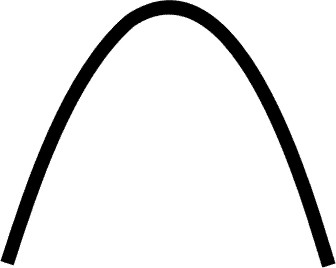
\includegraphics[width=0.300in,height= 0.300in]{flatxy1}}
\\ \hline
      &  &  \\
  +1  & Gaussian if \texttt{x>xloc}, flat (constant at the peak value) if \texttt{x<xloc}. &    
           {
\includegraphics[width=0.300in,height= 0.300in]{flatxy2}}
\\ \hline
      &  &  \\
  -1  & Gaussian if \texttt{x<xloc}, flat (constant at the peak value) if \texttt{x>xloc}. &    
           {
\includegraphics[width=0.300in,height= 0.300in]{flatxy3}}
\\ \hline

\end{longtable}

